%\tikzset{external/export next=false}
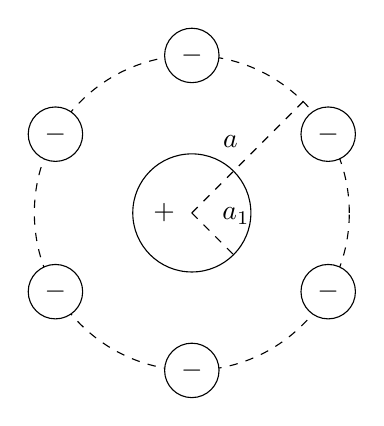
\begin{tikzpicture}
    % Inner Conductor
    \node [draw,circle,minimum width=1.5cm] at (0,0) {$+\qquad$};

    % Circle around which outer conductors are distributed
    \draw[dashed] (0,0) circle (2cm);

    % Outer conductors
    \foreach \angle in {30,90,150,210,270,330} {
        \node [fill=white,draw,circle] at (\angle:2) {$-$};
    }

    % Radii
    \draw[dashed] (0,0) -- node[midway,above left] {$a$} (45:2);
    \draw[dashed] (0,0) -- node[midway,above right] {$a_1$} (-45:0.75);
\end{tikzpicture}
